\chapter{Related Work} 
\label{Chapter3} 
\lhead{Chapter 3. \emph{Related Work}} 

\section{Native Client Acceleration Modules (NaClAM)} % (fold)
\label{sec:naclam}

In October 2012, John McCutchan at Google came up with the idea of using Native Client as a way to get native performance inside a normal JavaScript web application. He called it ``Native Client Acceleration Modules (NaClAM)'', with a slogan ``\emph{90\% Web App. Native Performance Where You Need It}''.

NaClAM is essentially a simple event-based RPC framework that allowed sending and receiving JavaScript objects as well as binary data. The RPC framework worked by using \emph{event listeners} and \emph{handlers} on both the JavaScript hand C++ ends. 

On the JavaScript side, a library called NaClAM.js was provided, which allowed developers to attach listeners to a particular module using the \lstinline{addEventListener(type,handler)} method. To send requests to the C++, the \lstinline{dispatchEvent} method is used. On the C++ side, messages are handled inside one overridden method called \lstinline{NaClAMModuleHandleMessage}. Here, checks are performed on the message received, and the appropriate method is called. Listing \ref{code_naclam_handle_message} shows an example of this. 

\lstset{language=C++,caption={NaClAM C++ message handler},label=code_naclam_handle_message}
\begin{code}
void NaClAMModuleHandleMessage(const NaClAMMessage& message) {
  if (message.cmdString.compare("floatsum") == 0) {
    handleFloatSum(message);
  } else if (message.cmdString.compare("addfloatarrays") == 0) {
    handleAddFloats(message);
  } else {
    NaClAMPrintf("Got message I don't understand");
  }
}
\end{code}

\subsection{Message Format} % (fold)
\label{sub:naclam_message_format}
\begin{figure}
	\centering
	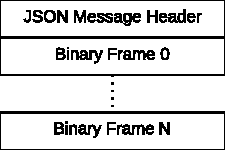
\includegraphics[width=0.3\textwidth]{naclam-msg-format.pdf} 
	\caption{A NaClAM message including binary frames}
	\label{fig:naclam_msg_format}
\end{figure}

At the message passing level, NaClAM uses JavaScript/C++ strings to transport messages. These messages hold information about the message such as the command string (like ``\lstinline{floatsum}'' in listing \ref{code_naclam_handle_message}). The strings are constructed using the jsoncpp library. 

Crucially, however, they also tell the framework how many binary \emph{frames} are expected to come after this message. Figure \ref{fig:naclam_msg_format} shows an example of a message containing $N$ frames. A frame is essentially a binary block of data sent by a separate call to \lstinline{PostMessage}. The receiver collects all the frames before triggering the event handler.

% subsection naclam_message_format (end)

\subsection{Advantages and Disadvantages} % (fold)
\label{sub:naclam_advantages_and_disadvantages}
NaClAM modules have the benefit of being simple and fast. There is a good distinction between the message information stored in the header and the message data stored as binary inside the frames. This allows developers to use the message header to implement event logic, while using the frames to transfer actual data. It also means that because the data is binary and almost no marshalling happens, the transfer speed is very fast, since binary data is \emph{shared} between JavaScript and C++.

However, there are a few issues with using NaClAM modules. The first is a lack of overall, high-level structure. The developer has to be aware and understand exactly what the framework is doing behind the scenes to write their application, which adds more burden on the developer, especially since almost no documentation is provided. The second issue is how the message header types are implemented. Although the framework allows sending application data in binary frames, the header information is sent as JSON, and is manipulated by the jsoncpp library - so another library the developer needs to get used to. Importantly, this means the developer needs to unpack and pack the data they are sending in the header section by themselves by using the jsoncpp library. Another issue is how the framework does not use a callback approach to asynchronous remote procedure calls. In other words, to `return' a value from a C++ function back to JavaScript, a \emph{different} event needs to be triggered from the C++, and handled by the JavaScript library. In other words, two different events need to be managed in both C++ and JavaScript for only one RPC call which returns data. If there are many functions like this, the developer needs to manage several different events, which is tedious. Finally, although the framework has been demoed and gained a lot of popularity, it still seems to not be well tested, as no unit tests exist for either the C++ or JavaScript implementations have been written. This makes it feel like an experimental project, rather than a full, well supported framework. 

Despite these issues, the Native Calls project was heavily influenced and inspired by the overall idea of the NaClAM project, especially its use cases and scenarios.
% subsection naclam_advantages_and_disadvantages (end)

% section naclam (end)

\section{Node.js C++ Addons} % (fold)
\label{sec:node_js_c_bindings}
Node.js is a JavaScript platform built on top of Chrome's V8 JavaScript engine that allows running JavaScript on server-side applications. Listing \ref{code_nodejs_http_server} shows an example of a node.js HTTP server.

\lstset{language=C,caption={A simple node.js HTTP server},label=code_nodejs_http_server}
\begin{code}
var http = require('http');
http.createServer(function (req, res) {
  res.writeHead(200, {'Content-Type': 'text/plain'});
  res.end('Hello World\n');
}).listen(1337, '127.0.0.1');
console.log('Server running at http://127.0.0.1:1337/');
\end{code}

Although the full JavaScript implementation is available to use in Node.js, it is possible to extend node.js by implementing addons. Addons are implemented using C++, and therefore allow developers to use efficient C++ functionality inside node.js. In fact, the C++ API allows you to wrap a C++ object with a JavaScript one. Listing \ref{code_nodejs_object_wrap_eg} shows an example of this.

\lstset{language=C++,caption={A node.js object wrapper},label=code_nodejs_object_wrap_eg}
\begin{code}
class MyObject : public node::ObjectWrap {
 public:
  static void Init(v8::Handle<v8::Object> exports);

 private:
  explicit MyObject(double value = 0);
  ~MyObject();

  static v8::Handle<v8::Value> New(const v8::Arguments& args);
  static v8::Handle<v8::Value> PlusOne(const v8::Arguments& args);
  static v8::Persistent<v8::Function> constructor;
  double value_;
};
\end{code}

In the \lstinline{Init} function, low level instructions that tell the JavaScript engine about the new object are given. In the \lstinline{New} member function, an instance of the C++ object is `wrapped' with the JavaScript object, using the node.js library. This means when we implement the \lstinline{PlusOne} method, we can `unwrap' the JavaScript object to get the C++ object instance, then perform the intended operation. Listing \ref{code_nodejs_wrapped_objects} shows how this works with the \lstinline{PlusOne} method.

\lstset{language=C++,caption={Implementing methods on wrapped objects},label=code_nodejs_wrapped_objects}
\begin{code}
Handle<Value> MyObject::PlusOne(const Arguments& args) {
  HandleScope scope;

  MyObject* obj = ObjectWrap::Unwrap<MyObject>(args.This());
  obj->value_ += 1;

  return scope.Close(Number::New(obj->value_));
}
\end{code}

Now, we can create an instance of the object in JavaScript as though it was a native JavaScript object. Listing \ref{code_nodejs_cpp_js_object} shows an example of this.

\lstset{language=C,caption={Using the C++ object from JavaScript},label=code_nodejs_cpp_js_object}
\begin{code}
var obj = new addon.MyObject(10);
console.log( obj.plusOne() ); // 11
console.log( obj.plusOne() ); // 12
\end{code}

\subsection{Advantages and Disadvantages} % (fold)
\label{sub:nodejs_cpp_advantages_and_disadvantages}
The idea of simply extending JavaScript to use your own C++ methods is powerful. We saw how the class we created in C++ can be accessed directly from JavaScript in a native way. It also means we have full control over the data the function can accept, as the actual JavaScript object reference is passed into the C++. In other words, there is no parameter marshalling - everything is native.

The obvious issue we have with C++ addons to JavaScript is how can we use them in \emph{browser} JavaScript? Well the answer is, we can't. However, we are able to set up a \emph{local} node.js server which we can communicate with using the browser. This can be done over the websocket protocol, which allow full-duplex communication over a single TCP connection. However, now the issue of parameter marshalling packing, and RPC comes to play. 


\subsection{Similar approaches in the browser} % (fold)
\label{sub:cpp_js_similar_approaches_in_the_browser}

% subsection cpp_js_similar_approaches_in_the_browser (end)
Although node.js addons do not actually solve our problem, the basic idea of them is that JavaScript is somehow \emph{extended} to allow running C++ functionality. Conventional browser plugins such as NPAPI based plugins or ActiveX browser plugins have similar interfaces. Through the plugin framework, it is possible to directly access the DOM on the page where the plugin is embedded - a bit like how this is done in node.js, as described above. 

Some frameworks such as FireBreath\footnote{\url{http://www.firebreath.org}} have been created that allow cross platform plugins that support ActiveX, NPAPI, etc. A crucial difference for us, however, is that these plugin frameworks depend on direct access to the DOM of the page in the browser. When we remove this feature, these frameworks will not work. Native Client \emph{only} allows access to the DOM through postMessage, and the data sent is \emph{passed by value}, so the data is essentially copied across to the C++ module. What this means is that the RPC framework will need to handle all marshalling as well as transport of the messages between C++ and JavaScript.
% subsection nodejs_cpp_advantages_and_disadvantages (end)

% section node_js_c_bindings (end)



\section{Apache Thrift: Cross-language services} % (fold)
\label{sec:apache_thrift_cross_language_services}
Apache Thrift is a framework that allows cross-language services development. Originally developed at Facebook, it was designed to provide reliable, efficient communication between languages and services. Many languages are supported, including C++, Java, and JavaScript. Thrift provides a cross-platform generator that can generate Thrift client and server pairs, where the client and server can be using different languages. Similar to other RPC frameworks, it uses its own IDL file format, Thrift IDL. The IDL file is used to generate code to support different languages.

\begin{figure}
    \centering
    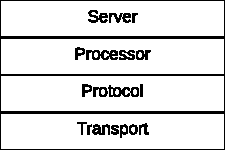
\includegraphics[width=0.3\textwidth]{thrift-stack.pdf} 
    \caption{The layers of the Apache Thrift RPC stack}
    \label{fig:thrift-stack}
\end{figure}

Thrift's implementation is based around layers in the thrift stack (Figure \ref{fig:thrift-stack}). The transport layer is responsible for the transfer of messages. The protocol layer is an interface that defines how certain data structures should be mapped into a transferable format, for example, JSON, XML, binary, etc. The process layer simply takes an input protocol, processes it using a handler, and writes to the output protocol. Finally the server sets up all the layers below it so that the system is functional as a whole.

In the following code listings, we give snippets showing how Apache Thrift is used to create a C++ server and JavaScript client. These were adapted from the original Thrift tutorial, which is available online\footnote{\url{http://thrift.apache.org/tutorial/}}.

\lstset{language=C++,caption={Thrift IDL File},label=code_thrift_idl_file}
\begin{lstlisting}
enum Operation {
  ADD = 1,
  SUBTRACT = 2,
  MULTIPLY = 3,
  DIVIDE = 4
}

struct Work {
  1: i32 num1 = 0,
  2: i32 num2,
  3: Operation op,
  4: optional string comment,
}

service Calculator extends shared.SharedService {
   void ping(),
   i32 add(1:i32 num1, 2:i32 num2),
   i32 calculate(1:i32 logid, 2:Work w)
}
\end{lstlisting}

\lstset{language=C++,caption={A Thrift C++ Server},label=code_thrift_cpp_server}
\begin{lstlisting}
class CalculatorHandler : public CalculatorIf {
 public:
  CalculatorHandler() {}

  int32_t add(const int32_t n1, const int32_t n2) {
    return n1 + n2;
  }

  int32_t calculate(const int32_t logid, const Work &work) {
    int32_t val;

    switch (work.op) {
    case Operation::ADD:
      val = work.num1 + work.num2;
      break;
    // ... other cases and implementation
    }
    return val;
  }

};

int main(int argc, char **argv) {
  // code here to set up processor, transport and protocol.

  TSimpleServer server(processor,
                       serverTransport,
                       transportFactory,
                       protocolFactory);


  server.serve();
  return 0;
}
\end{lstlisting}


\lstset{language=C,caption={JavaScript client for Thrift service},label=code_thrift_js_client}
\begin{lstlisting}
function calc() {
  var transport = new Thrift.Transport("/thrift/service/tutorial/");
  var protocol  = new Thrift.Protocol(transport);
  var client    = new CalculatorClient(protocol);

  var work = new Work()
  work.num1 = 1;
  work.num2 = 2;
  work.op = 1; //1==ADD

  var result = client.calculate(1, work);

  console.log(result); //3
  
}
\end{lstlisting}


\subsection{Advantages and Disadvantages} % (fold)
\label{sub:thrift_advantages_and_disadvantages}
Apache Thrift is a large library which seems to be well supported and used by both industry giants and the open source community. Because the Thrift IDL file is used to generate both clients and servers in more than a dozen languages, it seems that it is generic enough to be used in any language context. Thrift's implementation seems to be well structured, showing a clear separation of concerns between each component. 

However, there are a few issues with getting Thrift to work with Native Client. First, although it might be possible to implement a transport layer for thrift using postMessage in JavaScript, the C++ end (Native Client), writing a protocol for PPAPI might prove challenging. Moreover, the JSON protocol implementation uses strings instead of actual JSON objects, so this will probably impact performance, as it adds yet another marshalling step. For example, consider sending a JavaScript object from the web browser to a C++ function as a parameter. The marshalling will probably look something like this: we want to send a JavaScript Object, so Thrift for JavaScript will convert it into a JavaScript string in the protocol layer. When the JavaScript string is sent, it is marshalled by PPAPI as a \lstinline{pp::Var}, which is then marshalled as a \lstinline{std::string} using \lstinline{pp::Var::AsString()}. Thrift for C++ will then take this string and de-marshal it, in order to construct a C++ object. Finally, the C++ object is passed to the C++ concrete function. When we add on to this the fact that JavaScript strings are the slowest primitive types to transfer (according to our benchmarks in Section \ref{sec:performance_evaluation}, on page \pageref{sec:performance_evaluation}), we can see that the performance impact might actually make a big difference in an application. To avoid this, several changes will need to be made on many of the layers discussed above, which might prove to be a challenging, non-trivial task.

Finally, although unofficial port for Apache Thrift has been made for Native Client \footnote{\url{https://github.com/ahilss/thrift-nacl}}, all of the communication code is still hand coded. The performance of using Thrift for Native Client is unclear, as there is no protocol implemented using PPAPI.


% subsection thrift_advantages_and_disadvantages (end)

% section apache_thrift_cross_language_services (end)


\section{JSON-RPC Implementations} % (fold)
We briefly discussed the use of the JSON protocol RPC in background section \ref{sub:json_xml_rpc_intro} on page \pageref{sub:json_xml_rpc_intro}. Here, we discuss implementations of the protocol in JavaScript and C++.
\label{sec:json_rpc_implementations}


\subsection{JavaScript Implementations} % (fold)
\label{sub:pmrpc_json_rpc_using_postmessage}

In general, JavaScript implementations of the JSON RPC protocol are very simple, because JSON is consumed very naturally by the browser and JavaScript. Even if the JSON objects are sent and received as strings, implementations use the \lstinline{JSON.stringify(JSObject)} to turn a JavaScript object into a string, and \lstinline{JSON.parse(string)} to turn a string into a JavaScript object.

Although there are many implementations in JavaScript that are for several different domains and use cases, we discuss a simple one that uses \lstinline{postMessage} for transferring the JSON messages between browser windows, called ``PostMessage RPC (pmrpc)''. pmrpc is an open source library available on GitHub\footnote{\url{https://github.com/izuzak/pmrpc}} which aims to simplify cross-window communication by using postMessage. It shows the simplicity of remote procedure calls using JSON RPC. Listing \ref{code_prmpc_example} shows an example of using pmrpc to set up and call remote procedures between two windows.

\lstset{language=C,caption={Using pmrpc to communicate between two windows},label=code_prmpc_example}
\begin{code}
// in the callee window, expose a procedure
pmrpc.register({
  publicProcedureName : "HelloPMRPC",
  procedure : function(printParam) { alert(printParam); } 
});

// in the caller window, call the exposed procedure
pmrpc.call({
  destination : window.frames["ifr"],
  publicProcedureName : "HelloPMRPC",
  params : ["Hello World!"]
});
\end{code}
% subsection pmrpc_json_rpc_using_postmessage (end)

\subsection{C++ Implementations} % (fold)
\label{sub:jsonrpc_c_implementations}
C++ does not have native support for JSON like JavaScript, but several open source libraries exist that can read and  manipulate JSON strings. JsonCpp is one of the most popular JSON libraries for C++. We give a very brief overview of how it can be used to parse and write JSON objects. Listing \ref{code_jsoncpp_example} shows how JsonCpp is used.

\lstset{language=C++,caption={An example of using the JsonCpp library},label=code_jsoncpp_example}
\begin{code}
Json::Value root;   // will contain the root value after parsing.
Json::Reader reader;
bool parsingSuccessful = reader.parse( config_doc, root );

if(!parsingSuccessful){ /* fails to parse */ }

// Get the value of the member of root named 'encoding', 
// return 'UTF-8' if there is no such member.
std::string encoding = root.get("encoding", "UTF-8" ).asString();

// Get the value of the member of root named 'encoding', 
// return a 'null' value if there is no such member.

const Json::Value plugins = root["plug-ins"];
// Iterates over the sequence elements.
for ( int index = 0; index < plugins.size(); ++index )  
   loadPlugIn( plugins[index].asString() );
   
setIndentLength( root["indent"].get("length", 3).asInt() );
setIndentUseSpace( root["indent"].get("use_space", true).asBool() );

// don't need Json::Value constructor explicitly.
root["encoding"] = getCurrentEncoding();
root["indent"]["length"] = getCurrentIndentLength();
root["indent"]["use_space"] = getCurrentIndentUseSpace();

// jsoncpp to string
Json::StyledWriter writer;
std::string outputConfig = writer.write( root );
\end{code}

Notice how the API for JsonCpp is very similar to \lstinline{pp::Var} (see background section \ref{sub:using_PPAPI} on page \pageref{sub:using_PPAPI}). This is because \lstinline{pp::Var} and \lstinline{Json::Value} essentially do the same job - they are interfaces for JavaScript objects in C++. The crucial difference, however, is that \lstinline{Json::Value} ends up being written to a string, while \lstinline{pp::Var} objects are transferred as they are using PPAPI.

Now that we've looked at JsonCpp and how it is used, we look at an implementation of JSON RPC in C++ using JsonCpp called JsonRpc-Cpp\footnote{\url{http://jsonrpc-cpp.sourceforge.net/}}. Essentially, the framework will register methods using  the \lstinline{RpcMethod} class, which calls a function which accepts a \lstinline{Json::Value} input and a \lstinline{Json::Value} output passed by reference. Listing \ref{code_jsonrpccpphandler} shows an example of setting up a handler, adapted from the original documentation.

\lstset{language=C++,caption={Using a JsonRpc-Cpp handler},label=code_jsonrpccpphandler}
\begin{code}
class MyClass
{
   public:
     void Init()
     {
       RpcMethod* method = new RpcMethod<MyClass>(
           *this, &MyClass::RemoteMethod, // sets up pointer to C++ method
           std::string("remote_method"),  // the json-rpc "method"
           std::string("Description"));   // optional description
       m_handler.AddMethod(method);
     }

     bool RemoteMethod(const Json::Value& msg, Json::Value& response)
     {
       // do stuff
     }

   private:
     Handler m_handler;
};
\end{code}
% subsection jsonrpc_c_implementations (end)

\subsection{Advantages and Disadvantages} % (fold)
\label{sub:jsonrpc_advantages_and_disadvantages}
Many JSON RPC implementations for several languages exist\footnote{\url{http://en.wikipedia.org/wiki/JSON-RPC}}, including C++ and JavaScript as we have seen. The JSON-RPC protocol is very simple, and for most use cases, it is efficient and adequate. Although JSON RPC has a well defined protocol, it can be extended for specific implementations. Finally, JSON RPC does not need the messages to be sent and received as strings (although human-readability of the messages can be a bonus). We can use any other format to marshal and de-marshal a JSON RPC message. Some of these formats are discussed in background section \ref{sec:data_representation_and_transfer} on page \pageref{sec:data_representation_and_transfer}.

JSON RPC JavaScript implementations are simple enough to be implemented and tested in JavaScript to work for any specific project. So although libraries in JavaScript exist, implementing it for JavaScript to work with a different project structure / architecture should be not too difficult. As for C++ implementations, many if not all use the JsonCpp project. None available are implemented for \lstinline{pp::Var}. So to get JSON RPC to work with \lstinline{pp::Var}, an implementation will need to be written from scratch to use \lstinline{pp::Var}. This is also not too difficult, since as we've seen, \lstinline{Json::Value} and \lstinline{pp::Var} have similar APIs.

% subsection jsonrpc_advantages_and_disadvantages (end)

% section json_rpc_implementations (end)